%!TEX root = main.tex
%!TEX spellcheck = en_US 



\section{{Ekya}: Solution Description}
\label{sec:solution}







% Src: https://docs.google.com/drawings/d/1nBnwhi1agkQVHhFf01fLEV5nnQofWXlroUTv8ZCXxuw/edit?usp=sharing

% We start by formally defining our resource allocation problem (\S\ref{subsec:formulation}). In \S\ref{subsec:thief} and \S\ref{subsec:misc} we explain the design of our scheduling solution {\name} and its different features.

% We first formally define our joint retraining and inference with limited resource problem (\S\ref{subsec:formulation}). 
% We then explain the scheduling algorithm of \name (\S\ref{subsec:thief}) and how it estimates performance gains of various schedules (\S\ref{subsec:profiling}), before highlighting optimizations to address practical issues such as performance estimation errors (\S\ref{subsec:misc}).

%\subsection{Overview}
%\label{subsec:overview}


% overview
Continuous training on limited edge resources requires smartly deciding when to retrain each video stream's model, how much resources to allocate, and what configurations to use. Making these decisions presents two challenges.

First, the decision space of multi-dimensional configurations and resource allocations is computationally more complex than two fundamentally challenging problems of multi-dimensional knapsack and multi-armed bandits (\S\ref{subsec:formulation}). %, thus it is very expensive to explore the space of decisions. 
Hence, we design a {\bf thief scheduler} (\S\ref{subsec:thief}), 
% At the core of {\name} is its resource manager, that we refer to as 
a heuristic that makes the joint retraining-inference scheduling tractable in practice. % by exploring a relatively small yet beneficial fraction of the space of decisions. 
%We first formalize the joint retraining-inference scheduling under limited resource and analyze its complexity (\S\ref{subsec:formulation}). The thief scheduler makes the problem tractable in practice, by exploring a relatively small yet promising fraction of action space.
%, thus significantly reducing the problem complexity.

Second, the scheduler requires the model's exact performance (in resource usage and inference accuracy), but this requires retraining using all the configurations. 
%it is infeasible to know a model's exact performance (in resource usage and inference accuracy) for all retraining configurations, as it requires actual retraining and labeling using all configurations. However, this information is essential for the decision making.
We address this challenge with our {\bf micro-profiler} (\S\ref{subsec:profiling}), which retrains only a few select configurations on 
%which profiles the accuracies of many of retraining configurations by actually using them to retrain the model, but 
a fraction of the data. Figure \ref{fig:sys-arch} presents an overview of {\name}'s components. % with early termination.%, and does so only for a small number of promising configurations.  %and for a small number of training epochs, and then gradually prune the set of promising configurations. 

%To maximize the benefit of retraining, {\name}'s decision making and performance estimation must be fast and resource-efficient. 
%Our techniques (in \S\ref{subsec:thief} and \S\ref{subsec:profiling}) address both challenges. % drastically reduce the cost of decision making and performance estimation. %by at least two orders of magnitude when compared to \gaa{traditional solutions} while reaping the accuracy benefits from retraining. 
% to manage the inference and retraining of multiple videos at an edge server. 
% misc
%As shown, \name also includes practical solutions to a range of challenges in a continuous retraining system (\S\ref{subsec:misc}).



%We build upon the thief scheduler to support checkpointing of models {\em during} retraining (\S\ref{subsubsec:checkpoint}) to provide the inference with more accurate models sooner. 
%{\name} also {\em dynamically reallocates resources} when it detects errors in the resource-accuracy estimations (\S\ref{subsubsec:error-profiles}). %We describe the other factors that impact continuous training in \S\ref{subsec:misc}. 
%Generating the resource-accuracy estimations of the retraining jobs is described in \S\ref{sec:profiling}.


%\begin{table}[t!]
\small
\begin{tabular}{cl}
{\bf Notation} & {\bf Description}\\\hline
$V$ & Set of video cameras\\
$v$ & Single video camera\\\hline
$G$ & Total GPU resources\\
$g^v_R$ & Resources for retraining video stream $v$\\
$g^v_I$ & Resource for inference on video stream $v$\\\hline
$\Gamma_v$ & Set of all configurations for retraining $v$\\
 & (each configuration is referred to as $\gamma_v$)\\
$\Lambda_v$ & Set of all configurations for inference on $v$\\
 & (each configuration is referred to as $\lambda_v$)\\\hline
$a_v$ & Accuracy of inference on video stream $v$\\
$\alpha_v$ & Accuracy of inference over time window\\
$T$ & Retraining window duration\\\hline\\
\end{tabular}
\caption{\label{tab:notations}\small\bf Notations used in {\name}'s description.}
\end{table}

\subsection{\hspace{-0.2cm}Formulation of joint inference-retraining scheduling}
\label{subsec:formulation}
% Setup
We maximize the inference accuracy of all video streams in a retraining window. Table \ref{tab:notations} has the list of relevant notations.
We consider a pool of edge GPUs $G$ (each edge server might have a few GPUs~\cite{azure-ase}) shared by the inference and retraining jobs of a set of video streams $V$, with video $v$($\in V$)'s inference job getting $g^{v}_I$ GPU resources and its training job getting $g^{v}_R$ GPU resources\footnote{\junchen{need to clarify why we only share GPU cycles, not RAM, etc.}}. 
For each video $v \in V$, we denote its inference accuracy $a_v$, which could be improved by retraining.
$\gamma_v$ is the retraining configuration, picked from a pool of \textit{configurations} $\Gamma_v$, to retrain the model of video $v$.
$\lambda_v$ is the inference configuration (e.g., frame sampling rate), picked from an inference resource-accuracy profile $\Lambda_v$ \cite{videostorm, chameleon}, to run the inference job of video $v$.
Note that inference configurations are always chosen such that its resource demand does not exceed the allocation $g^v_I$ for inference.

Given the retraining and inference configurations ($\gamma_v,\lambda_v$) and resource allocations ($g^{v}_R, g^{v}_I$) of a video $v$, its inference accuracy at time $t$ is
$a_v(t, g^v_R, \gamma_v, g^v_I, \lambda_v)$ and inference accuracy measured over the retraining window $T$ can be expressed by 
\[
\alpha_v (T) = \frac{1}{T} \int_{t=0}^{T} a_v(t, g^v_R, \gamma_v, g^v_I, \lambda_v)\ dt
\]


%Edge deployments have one or few edge servers that have multiple video cameras $V$ streaming to them for analytics (\S\ref{subsec:edge}). The analytics on the video streams in $V$ share the same GPU resource pool $G$ (typically, a few GPUs per edge server \cite{azure-ase}). For each video stream $v \in V$, there is a continuous inference job whose inference accuracy is $a_v$. A retraining job is run periodically per video stream which improves $a_v$. The resource pool $G$ must be split across the inference and retraining jobs of all video streams, with video $v$'s inference job getting $g^{v}_I$ GPU resources and its training job getting $g^{v}_R$ GPU resources. Table \ref{tab:notations} has the list of relevant notations.



% Training Profiles. Not going into details on how performance scales with resources..
%Every retraining job of video $v$ has a pool of \textit{configurations} $\Gamma_v$ (\S\ref{subsec:profiles}). Each configuration $\gamma_v \in \Gamma_v$ specifies the hyperparameters and an associated accuracy-resource\_time profile. Increased resource allocation to training grants more resource\_time to the training job, allowing it to achieve a higher accuracy for the same wall\_time. Once a retraining job completes, it updates the inference job with the new model. Similar to the training configurations, the inference job of each camera $c$ has a inference performance profile, which dictates the scaling of the inference accuracy as the inference resource allocation changes.
%\noindent{\bf Configurations:} Every retraining job of video $v$ has a pool of \textit{configurations} $\Gamma_v$. Each configuration $\gamma_v \in \Gamma_v$ specifies the hyperparameters and its accuracy (see \S\ref{subsec:profiles}). Increasing resource allocation to retraining ($g^v_R$) allows it complete faster and update the inference job sooner with the new model.% with higher accuracy. 
%
%The inference job of each video stream $v$ also has a resource-accuracy profile $\Lambda_v$ \cite{videostorm, chameleon}, with each configuration $\lambda_v \in \Lambda_v$ (e.g., frame sampling rate) in the profile specifying the current inference accuracy ($a_v$) as well as the resource {\em demand} to keep up with the processing of the live video stream. %All the inference configurations can keep up with processing the live video stream if its corresponding resource demand is allocated, but their accuracies will vary. % which dictates the scaling of the inference accuracy as the inference resource allocation changes.
%Inference configurations are always chosen such that its resource demand does not exceed the allocation $g^v_I$ for inference.

% Define inference accuracy.
%\noindent{\bf Inference accuracy over time:} 
%The inference accuracy of a video $v$ measured over the retraining window depends on the inference configuration (which in turn depends on its resources allocation $g^v_I$) as well as the inference model (pre-retraining and post-retraining). The accuracy of the model post-retraining depends on the retraining configuration $\gamma_v \in \Gamma_v$ and the GPU allocation to the retraining $g^v_R$. Thus, for a video stream $v$ whose inference accuracy at any point in time is $a_v$, the inference accuracy $\alpha_v$ averaged over time $t=0 \rightarrow T$ is (where $T$ is the retraining window):
%\[
%\alpha_v (T) = \frac{1}{T} \int_{t=0}^{T} a_v(t, g^v_R, \gamma_v, g^v_I, \lambda_v)\ dt
%\]

% Objective - What are the metrics and why
\noindent The joint retraining-inference optimization maximizes the average accuracy over a retraining window across all videos through selecting configurations ($\gamma_v$ and $\lambda_v$) and allocating resource between retraining ($g^{R}_v$) and inference ($g^{I}_v$):
\begin{equation}
    \begin{aligned}
        & \underset{g_{R}^v, g_{I}^v, \gamma_v, \lambda_v}{\text{maximize}}
        %& & \frac{\sum_{v \in V}\alpha_v(T, g_{R}^v, \gamma_v, g_{I}^v, \lambda_v)}{|V|} \\
        & & \frac{\sum_{v \in V}\alpha_v(T)}{|V|} \\
        & \text{s.t.}
        & & \sum_{v \in V} g_{R}^v + g_{I}^v \leq G\\
        %&&& a_v(t, g_{R}^v, \gamma_v, g_{I}^v, \lambda_v) \geq a_\text{MIN} \\
        &&& a_v(t) \geq a_\text{MIN}, \forall v \in V, 0 \leq t \leq T 
        %TODO(romilb): Cleanup this min accuracy expression
    \end{aligned}
    \label{eqn:optimization}
\end{equation}
The joint retraining-inference scheduling essentially balances the inference accuracy before retraining finishes and the optimization of long-term accuracy by finishing model retraining as soon as possible.
This fundamentally differs from optimization for only inference accuracy or only training accuracy in two aspects.
Additionally, we allow for the inference accuracy $a_v$ at any point in time to be bounded by a minimum $a_\text{MIN}$ (application-specific bound), so that the inference results remain useful to the application, especially when the model is being retrained.


%As shown in \S\ref{subsec:motivation-sched-example}, optimizing for only the inference accuracy or only the retraining accuracy does not maximize the inference accuracy over the retraining window, $\alpha_v (T)$. % over all cameras $v \in V$. 
%%optimizing for maximum training accuracy is immaterial since the goal is not just to retrain the model, but also use it while it is still useful. Thus the objective is to maximize the mean inference accuracy across all cameras $C$ present in the system by picking the correct configurations and resource allocations, constrained by the size of the resource pool available.
%% https://jcnts.wordpress.com/2009/11/11/formatting-optimization-problems-with-latex/
%%\noindent{\bf Optimization formulation:} 
%
%We seek to maximize the average inference accuracy over the retraining window $T$ (i.e., $\alpha_v(T)$) across all videos $v \in V$ by picking the configurations $\gamma_v$ and $\lambda_v$ for each video stream $v$'s retraining and inference, and allocating the edge's GPU resource $G$ for retraining ($g^{R}_v$) and inference ($g^{I}_v$). Additionally, we allow for the inference accuracy $a_v$ at any point in time to be bounded by a minimum $a_\text{MIN}$ (application-specific bound), so that the inference results remain useful to the application.

% computationally intractable
\mypara{Complexity analysis}
The complexity of the above optimization is combinatorial in the number of configurations and cameras. As a result, we proceed to devise an efficient scheduling heuristic.% that provides good results in practice.
\junchen{Kevin, the complexity discussion can be here}






\subsection{Formulation of joint inference and retraining}
\label{subsec:formulation}

The problem of joint inference and retraining aims to maximize overall inference accuracy for all video streams $\mathcal{V}$ in a retraining window ${T}$ with duration $\lVert T \rVert$. 
All work must be done in $\mathcal{G}$ GPUs.
Thus, the total compute capability is $\mathcal{G}\lVert T \rVert$ GPU-time. Without loss of generality, let $\delta$ be the smallest granularity of GPU allocation.  %(e.g., if $\delta = 1\%$ of GPU, $150\delta =$ 1.5 GPU). Let $\Theta$ be the set of all possible GPU allocations $\Theta = \{0, 1, ..., \frac{\mathcal{G}}{\delta}\}$.
Each video $v \in V$ has a set of \emph{retraining} configurations $\Gamma$
and a set of \emph{inference} configurations $\Lambda$ (\S\ref{subsec:profiles}).
Table \ref{tab:notations} (\S{\ref{appendix:scheduler}}) lists the notations. 



\noindent\textbf{Decisions.} For each video $v\in\mathcal{V}$ in a window $T$, we decide: (1) the retraining configuration $\gamma\in\Gamma$ ($\gamma = \emptyset$ means no retraining); (2) the inference configuration $\lambda\in\Lambda$; and (3) how many GPUs (in multiples of $\delta$) % (in terms of GPU resource units $\delta$)
to allocate for retraining ($\mathcal{R}$) %\in\Theta$) 
and inference ($\mathcal{I}$). %\in\Theta$). 
We use binary variables $\phi_{v\gamma\lambda\mathcal{R}\mathcal{I}}\in\{0,1\}$ to denote these decisions (see Table \ref{tab:notations} \S{\ref{appendix:scheduler}} for the definition). 
These decisions require $C_T(v, \gamma, \lambda)$ GPU-time and yields overall accuracy of $A_T(v, \gamma, \lambda, \mathcal{R}, \mathcal{I})$. $A_T(v, \gamma, \lambda, \mathcal{R}, \mathcal{I})$ is averaged across the window $T$ (\S\ref{subsec:motivation-sched-example}), and the above decisions determine the inference accuracy at {\em each point in time}.
%Specifically, let $a_t(v, \gamma, \lambda, \mathcal{R}, \mathcal{I})$ be the inference accuracy for video $v$ at a point in time $t$, % given retraining configuration $\gamma$, inference configuration $\lambda$, $\mathcal{R}\delta$ GPUs for retraining, and $\mathcal{I}\delta$ GPUs for inference, we have:
%\[
%\ A_T(v, \gamma, \lambda, \mathcal{R}, \mathcal{I}) = 
%\frac{1}{\lVert T \rVert} \int_{t=0}^{\lVert T \rVert} a_t(v, \gamma, \lambda, \mathcal{R}, \mathcal{I})\ dt
%\]


%At each retraining window $t \in \mathcal{T}$, the system maintains a set of DNN instances $M_{v}^t$ for video $v$, where each $m_{v\gamma}^t \in M_{v}^t$ denotes a DNN instance that is trained based on configuration $\gamma$. Each DNN $m_{v\gamma}^0 \in M_{v}^0$ is pretrained with offline video data. 
%The system can optionally retrain $m_{v\gamma}^t$ into $\hat{m}_{v\gamma}^t$ with training configuration $\gamma$ and the video data of $v$ at $t$, and the retraining cost is $C^R(v, t, \gamma)$.

%The system must pick a DNN $m_{v\gamma}^t$ or $\hat{m}_{v\gamma}^t$ and an inference configuration $\lambda \in \Lambda$ to run inference for video $v$ at $t$.
%The inference cost of such a decision is $C^I(v, t, \gamma, \lambda$), and the inference accuracy is $A(v, t, m, \lambda)$ where $m$ is the chosen DNN. 
%We use binary variables $r_{vt\gamma g}$ and $i_{vt\gamma \lambda g}$ to indicate the decisions made by the system (see Table \ref{tab:notations} for their definitions).

\noindent\textbf{Optimization.} Maximize the inference accuracy averaged across all videos in a retraining window within the GPU limit. 

{\small
\vspace{-12pt}
\begin{equation}
    \begin{aligned}
    %\footnotesize
       & \underset{\phi_{v\gamma\lambda\mathcal{R}\mathcal{I}}}{\arg\max}
         \frac{1}{\lVert \mathcal{V} \rVert}
         \sum_{\substack{\forall v\in\mathcal{V}, 
                        \forall \gamma\in\Gamma,
                        \forall \lambda\in\Lambda,\\
                        \forall \mathcal{R}, \forall \mathcal{I} \in \{0, 1, ..., \frac{\mathcal{G}}{\delta}\} %\in \Theta,
                        %\forall \mathcal{I} \in \Theta
                        }}
          \phi_{v\gamma\lambda\mathcal{R}\mathcal{I}} \cdot
          A_T(v, \gamma, \lambda, \mathcal{R}, \mathcal{I})\\
       & \text{subject to}\\
       & 1. \sum_{\substack{\forall v\in\mathcal{V}, 
                        \forall \gamma\in\Gamma,
                        \forall \lambda\in\Lambda,\\
                        \forall \mathcal{R}, \forall \mathcal{I}}}
                        \phi_{v\gamma\lambda\mathcal{R}\mathcal{I}} \cdot
                        C_T(v, \gamma, \lambda)
                        \leq \mathcal{G}\lVert T \rVert \\
      & 2. \sum_{\substack{\forall v\in\mathcal{V},
                        \forall \gamma\in\Gamma,
                        \forall \lambda\in\Lambda,\\
                        \forall \mathcal{R}, \forall \mathcal{I}}}
                           \phi_{v\gamma\lambda\mathcal{R}\mathcal{I}} \cdot
                           (\mathcal{R} + \mathcal{I})
                        \leq \frac{\mathcal{G}}{\delta} \\
      & 3. \sum_{\substack{\forall \gamma\in\Gamma, 
                           \forall \lambda\in\Lambda,\\ 
                           \forall \mathcal{R}, %\in \Theta,
                           \forall \mathcal{I}}} %\in \Theta}}
           \phi_{v\gamma\lambda\mathcal{R}\mathcal{I}} \leq 1, 
           \forall v\in\mathcal{V}
    \end{aligned}
    \label{eqn:optimization}
\end{equation}
}%

The first constraint ensures that the GPU allocation does not exceed the available GPU-time $\mathcal{G}\lVert T \rVert$ in the retraining window. The second constraint limits the {\em instantaneous}  allocation (in multiples of $\delta$) to never exceed the available GPUs. 
%The third constraint ensures that the system can only pick at most one retraining configuration/allocation and one inference configuration/allocation for each video $v$.
The third constraint ensures that at most one configuration is picked for retraining and inference each for a video $v$.





% https://docs.google.com/drawings/d/1nBnwhi1agkQVHhFf01fLEV5nnQofWXlroUTv8ZCXxuw/edit?usp=sharing
%\begin{figure*}[t!]
%    \centering
%    \includegraphics[width=0.85\linewidth]{ekya/figures/Solution/"Ekya System Architecture Arch".pdf}
%    \caption{{\name} System Architecture. \ga{Make it a one-column figure.}}
%    \label{fig:sys-arch}
%\end{figure*}

% % rest of the section
% \subsection{Solution Overview}
% \label{subsec:overview}

% Figure \ref{fig:sys-arch} presents an overview of {\name} to manage the inference and retraining of videos at an edge server. At the core of {\name} is its resource manager, that we refer to as ``thief'' scheduler, which is a greedy scheduling heuristic (\S\ref{subsec:thief}). We build upon the thief scheduler to support checkpointing of models {\em during} retraining (\S\ref{subsubsec:checkpoint}) to provide the inference with more accurate models sooner. {\name} also {\em dynamically reallocates resources} when it detects errors in the resource-accuracy estimations (\S\ref{subsubsec:error-profiles}). %We describe the other factors that impact continuous training in \S\ref{subsec:misc}. 
% Generating the resource-accuracy estimations of the retraining jobs is described in \S\ref{sec:profiling}.
%\revtext{This optimization problem can be expressed as a multi-dimensional binary knapsack problem while the uncertainty of $A_T(v, \gamma, \lambda, \mathcal{R}, \mathcal{I})$ can be modelled as multi-armed bandits (MAB) problem. A detailed complexity analysis is presented in \S\ref{complexity-analysis}.}
Our analysis in \S\ref{complexity-analysis} shows that the above optimization problem is {\em harder} than the multi-dimensional binary knapsack problem and modeling the uncertainty of $A_T(v, \gamma, \lambda, \mathcal{R}, \mathcal{I})$ is more challenging than the multi-armed bandit problem.
%\ga{Summarize the complexity analysis.}


\begin{figure}[t]
    \centering
    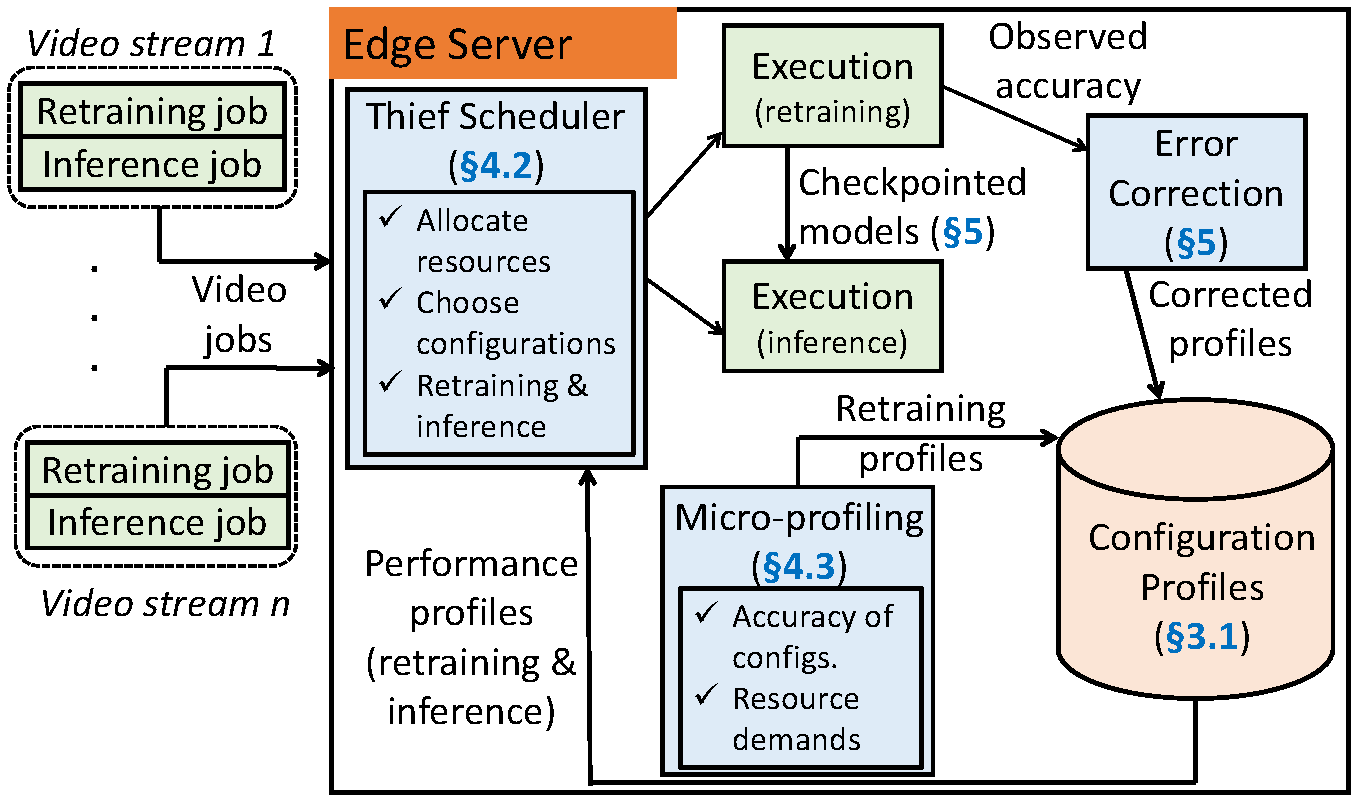
\includegraphics[width=.85\columnwidth]{ekya/figures/overview_cropped.pdf}
    \caption{\small\bf {\name}'s components and their interactions. }%\ga{Update with the right section numbers.}}
    \label{fig:sys-arch}
\end{figure}

\subsection{Thief Scheduler}
\label{subsec:thief}




%The computational intractability of the formulation in \S\ref{subsec:formulation} stems primarily from jointly allocating resources and picking configurations. In this section, we decouple the two and develop an efficient and iterative heuristic (Algorithm \ref{algo:thief_sched}). 
Our scheduling heuristic makes the scheduling problem tractable by decoupling resource allocation (i.e., $\mathcal{R}$ and $\mathcal{I}$) and configuration selection (i.e., $\gamma$ and $\lambda$) (Algorithm \ref{algo:thief_sched}). %It iteratively allocates resources to all inference and retraining jobs and picks inference/retraining configurations within the limit of the allocated resource. 
%We present the heuristic and then explain the key assumptions and relaxations that it is built upon. 
%\textbf{Challenge:} Equation \ref{eqn:optimization} requires that both the resource allocation and the configurations must be picked jointly. One influences the other, thus we present an iterative algorithm \ref{algo:thief_sched} which tries to converge on the optimal (?) combination.
We refer to {\name}'s scheduler as the ``thief'' scheduler and it iterates among all inference and retraining jobs as follows.% and picks inference/retraining configurations within the limit of the allocated resource. %configuration selection as follows. 
%\begin{packeditemize}

%\item 
{\bf (1)} It starts with a fair allocation for all video streams $v \in V$ (line 2 in Algorithm \ref{algo:thief_sched}). 
In each step, it iterates over all the inference and retraining jobs of each video stream (lines 5-6), and {\em steals} a tiny quantum $\Delta$ of resources (in multiples of $\delta$; see Table \ref{tab:notations}, \S\ref{appendix:scheduler}) from each of the other jobs (lines 10-11).

%\item 
{\bf (2)} With the new resource allocations ({\small temp\_alloc[]}), it then selects configurations for the jobs using the {\sf\footnotesize PickConfigs} method (line 14 and Algorithm \ref{algo:pickconfigs}, \S{\ref{appendix:scheduler}}) that iterates over all the configurations for inference and retraining for each video stream.  
For inference jobs, among all the configurations whose accuracy is $\geq a_\text{MIN}$, {\sf\footnotesize PickConfigs} picks the configuration with the highest accuracy that can keep up with the inference of the live video stream given current allocation (line 3-4, Algorithm \ref{algo:pickconfigs}, \S{\ref{appendix:scheduler}}).  

For retraining jobs, {\sf\footnotesize PickConfigs} picks the configuration that maximizes the accuracy $A_T(v, \gamma, \lambda, \mathcal{R}, \mathcal{I})$ over the retraining window for each video $v$ (lines 6-12, Algorithm \ref{algo:pickconfigs}, \S{\ref{appendix:scheduler}}). {\sf\footnotesize EstimateAccuracy} (line 7, Algorithm \ref{algo:pickconfigs}, \S\ref{appendix:scheduler}) aggregates the instantaneous accuracies over the retraining window for a given pair of inference configuration (chosen above) and retraining configuration. {\name}'s micro-profiler (\S\ref{subsec:profiling}) provides the estimate of the accuracy and the time to retrain for a retraining configuration when $100\%$ of GPU is allocated, and {\sf\footnotesize EstimateAccuracy} proportionately scales the GPU-time for the current allocation (in {\small temp\_alloc[]}) and training data size. In doing so, it avoids configurations whose retraining durations exceed $\lVert T \rVert$ with the current allocation (first constraint in Eq. \ref{eqn:optimization}). %, while ensuring the total compute cost does not exceed the total GPU time. 
%\S\ref{subsec:profiling} explains how we estimate the accuracy of retraining and \gaa{time to retrain} with each configuration. %\footnote{\S\ref{subsec:profiling} estimates the time to retrain when $100\%$ of the GPU is allocated to the retraining, and we linearly estimate the time taken to retrain for any given allocation and training data size inside {\sf PickConfigurations}.}
%We proportionately scale the GPU-time for any given allocation and training data size in {\sf\footnotesize PickConfigs}. \S\ref{subsec:profiling} explains how we estimate the accuracy of retraining and the time to retrain when $100\%$ of the GPU is allocated. 

% {\sf\small PickConfigurations} only checks the Pareto boundary of configurations (Figure \ref{fig:resource-profiles}). 

%\item
{\bf (3)} After reassigning the configurations, {\name} uses the estimated average inference accuracy (accuracy\_avg) over the retraining window (line 14 in Algorithm \ref{algo:thief_sched}) and keeps the new allocations only if it improves up on the accuracy from prior to stealing the resources (line 15 in Algorithm \ref{algo:thief_sched}).

%using {\sf\small Estim} (line 14). 
% the accuracy after stealing resources is higher than the accuracy prior to the stealing (line 14).
%\end{packeditemize}
%steals an additional quantum $\delta$ for the {\small thief\_job} 
%The performance estimation module ({\sf\small Estim}) can produce the $\alpha_v(T)$ for all the video streams $v \in V$ with any given configuration and resource allocation, and we will explain it in next in \S\ref{subsec:profiling}.


The thief scheduler repeats the process till the accuracy stops increasing (lines 15-20 in Algorithm \ref{algo:thief_sched}) and until all the jobs have played the ``thief''. 
Algorithm~\ref{algo:thief_sched} is invoked at the beginning of each retraining window, as well as on the completion of every training job during the window.% to reallocate resources to the other training and inference jobs.

% \begin{algorithm}
%  \KwData{Configuration profiles $\Gamma_v$ and $\Lambda_v$ and resource allocations $g^{c}_R$ and $g^{c}_I$ for video $v$}
%  \KwResult{The optimal configurations $\gamma^{opt}_{v}$ and  $\lambda^{opt}_{v}$}
%  
%  best\_accuracy = 0\;
%  \For{$\lambda_v$ in $\Lambda_v$}{
%     \For{$\gamma_v$ in $\Gamma_v$}{
%          accuracy = simulator([$\lambda_v$, $\gamma_v$], [$g^{c}_R$, $g^{c}_I$])\;
%         \If{accuracy > best\_accuracy}{
%             $\lambda^{opt}_{v}$, $\gamma^{opt}_{v}$ = $\lambda_v$, $\gamma_v$\;
%             best\_accuracy = accuracy\;
%         }
%     }
%  }
% 
% return $\lambda^{opt}_{v}$, $\gamma^{opt}_{v}$\;
% \caption{ConfigurationPickingRoutine}
% \label{algo:config_pick}
%\end{algorithm}

\begin{algorithm}[t]
\small
\KwData{Training ($\Gamma$) and inference ($\Lambda$) configurations}
\KwResult{GPU allocations $\mathcal{R}$ and $\mathcal{I}$, chosen configurations ($\gamma \in \Gamma$, $\lambda \in \Lambda$) $\forall v \in V$}% for the period T.}
 
 % Run in a loop to do iterations of configuration selection and resource allocation
all\_jobs[] = Union of inference and training jobs of videos $V$\;
\tcc{Initialize with fair allocation}
 best\_alloc[] = fair\_allocation(all\_jobs)\; 
% \For{iteration in iteration\_count}{
     % Perform SCO - Single camera optimization which picks the best hyperparameters.
%     \For{v in V}{
%        v.training\_config = {\sf\footnotesize PickConfigurations}(v, curr\_alloc[v]) \;
%     }
 best\_configs[], best\_accuracy\_avg =  {\sf\footnotesize PickConfigs}(best\_alloc)\;
     % Perform thief resource stealing
     \tcc{Thief resource stealing}
%     best\_accuracy\_avg = 0\;
     \For{\text{\em thief\_job} in \text{\em all\_jobs[]}}{
        \For{\text{\em victim\_job} in \text{\em all\_jobs[]}}{
            \lIf{\text{\em thief\_job} == \text{\em victim\_job}} {\bf continue}
            temp\_alloc[] $\leftarrow$ best\_alloc[]\;
            \While{true}{
                \tcc{$\Delta$ is the increment of stealing}
                temp\_alloc[victim\_job] $-$= $\Delta$\;
                temp\_alloc[thief\_job] $+$= $\Delta$\;
                \lIf{{\em temp\_alloc[victim\_job]} < {\em 0}}{
                    \bf break
                }
                \tcc{Calculate accuracy over retraining window and pick configurations.}temp\_configs[], accuracy\_avg = {\sf\footnotesize PickConfigs}(temp\_alloc[])\;
                %\tcc{Calculate accuracy over retraining window and pick configurations.}%accuracy\_$\alpha$ = {\sf\footnotesize Estim}(temp\_configs[], temp\_alloc[])\;
                \If{{\em accuracy\_avg} > {\em best\_accuracy\_avg}}{
                    best\_alloc[] = temp\_alloc[]\;
                    best\_accuracy\_avg = accuracy\_avg\;
                    best\_configs[] = temp\_configs[];
                }
                \Else{\bf break\;}
            }
        }
     }
% }
 {\bf return} {best\_alloc[], best\_configs[]}\;
 
 \caption{Thief Scheduler.
 %\junchen{it's going through all the users, rather than iterative algorithm.. may need a better structure}
 %\romil{Explain estim in function call.}
 }
 \label{algo:thief_sched}
\end{algorithm}










%% PickConfigurations
% For the given allocation, finds the best configuration and returns the accuracy gotten by the best configuration and given resource allocation.

\begin{algorithm}[t]
\small
 \KwData{Resource allocations in {temp\_alloc[]}, configurations ($\Gamma$ and $\Lambda$), retraining window $T$, videos $V$}
 \KwResult{Chosen configs $\forall v \in V$, %for the given $\mathcal{R}^\prime$ and $\mathcal{I}^\prime$, 
 average accuracy over $T$}
 
     chosen\_accuracies[] $\leftarrow$\{\}; chosen\_configs[] $\leftarrow$\{\}\;
     \For{\text{\em v} in $V$\text{\em []}}{
        %\tcc{Pick highest accuracy inference cfg}
        infer\_config\_pool[] = $\Lambda$.{\bf where}(\text{resource\_cost} < temp\_alloc[v.inference\_job] \&\& accuracy $\geq a_\text{MIN}$ )\;
        % Add alpha min filter in cfg_pool
        infer\_config = {\bf max}(infer\_config\_pool, {\bf key}=accuracy)\;
        %\tcc{Pick training configuration}
        best\_accuracy = 0\;
        % best\_training\_cfg = None\;
        \For{\text{\em train\_config} in \text{\em $\Gamma$}}{
            \tcc{Estimate accuracy of inference/training config pair over retraining window} % Done using profiles.
            accuracy = {\sf\footnotesize EstimateAccuracy}(train\_config, infer\_config, temp\_alloc[v.training\_job], $T$)\;
            \If{\text{\em accuracy} > \text{\em best\_accuracy}} {
                best\_accuracy = accuracy\;
                best\_train\_config = train\_config\;
            }
        }
        chosen\_accuracies[v] = best\_accuracy\;
        chosen\_configs[v] = \{infer\_config, best\_train\_config\}\;
     }
    {\bf return} chosen\_configs[], {\bf mean}(chosen\_accuracies[])\;
 
 \caption{\bf\small PickConfigs}
 \label{algo:pickconfigs}
\end{algorithm}

%{\name}'s scheduler starts with a {\em fair} resource allocation for all video streams $v \in V$; for any given resource allocation (of a retraining or inference job), it picks the configuration with the highest accuracy but whose resource demand is less than the allocation. % which maximize inference accuracy for this period. The configurations are picked by the configuration picking routine (\cref{algo:hyperparam_pick}), which uses the simulator $S$ to exhaustively evaluate all training configurations $\gamma_v \in \Gamma_v$ and inference configurations $\lambda_v \in \Lambda_v$ for all video streams $v \in V$.

%After picking the configurations for the given fair resource allocation, the thief allocator iterates over every job, steals a tiny quantum of resource from the remaining jobs and evaluates the accuracy this resource allocation with the simulator $S$. If the accuracy increases, it tries stealing more resources till accuracy stops increasing. It then moves to the next job and repeats till all jobs have played the "thief" and arrived at the maximum pareto accuracy. Once this is done, the thief scheduler re-evaluates the hyperparameter configurations with the algorithm to verify if the current selection is optimal for the new resource allocation. If it is, the algorithm terminates. Else, new hyperparameters are selected and the process is repeated.



\mypara{Design rationale} 
We call out the key aspects that makes the scheduler's decision efficient by pruning the search space. %improves its efficiency while potentially introducing sub-optimality to its decisions.
%starting sequence of jobs
%\item {\em Iterating through the jobs only once:} The thief scheduler orders the jobs ({\sf\small all\_jobs}) in descending order of the expected improvement in accuracy (\ie accuracy after the retraining compared to its current accuracy).  This prioritizes jobs with the most improvement to play the ``thief'' and give them more resource first, while ensuring a bounded computational complexity of the thief scheduler.

\begin{itemize}
%quantum of resource increments
\item {\em Coarse allocations:}
The thief scheduler allocates GPU resources in quantums of $\Delta$. \revtext{Intuitively, $\Delta$ is the step size for allocation used by the scheduler. 
Thus, the final resource allocation from the thief scheduler is within $\Delta$ of the optimal allocation.} 
% This makes the thief scheduler arrive at a resource allocation within $\Delta$ of the optimal allocation.} 
We empirically pick a $\Delta$ that is coarse yet accurate enough in practice, while being mindful of modern GPUs\cite{nvidia-mps}; see \S\ref{subsec:eval-understanding}. %We analyze the sensitivity of $\Delta$ in \S\ref{subsec:eval-understanding}. 
Algorithm \ref{algo:thief_sched} ensures that the total allocation is within the limit (second constraint in Eq~\ref{eqn:optimization}). %The smaller the $\Delta$ the closer to optimal is our allocation, but also inefficient to compute. The quantum $\Delta$ is an experimental parameter whose sensitivity we vary in \S\ref{subsec:sensitivity-eval}.

%starting resource allocations
%\item {\em Starting with a fair resource allocations:}As the decision space for GPU resource allocation ($\mathcal{R}$ and $\mathcal{I}$ $\forall v \in \mathcal{V}$) is very large, we start our exploration with the fair allocation. While other initial allocations can also be used, we seek to improve upon the baseline of fair allocations. 

%temporal switch only on job completions
\item {\em Reallocating resources only when a retraining job completes:}
% , but otherwise the thief scheduler does not temporally vary the allocations among running jobs. 
Although one can reallocate GPU resource among jobs at finer temporal granularity (\eg whenever a retraining job has reached a high accuracy), we empirically find that the gains from such complexity is marginal. %further optimizations does not commensurate the added system complexity.
%That said, \name periodically checkpoints the model so that inference can get the up-to-date accuracy from retraining.
% we partially mitigate this drawback in \S\ref{subsubsec:checkpoint} by periodically {\em checkpointing} the model during the retraining and reallocating resources after each checkpoint.

\item{\em Pruned configuration list:} 
Our micro-profiler (described next) speeds up the thief scheduler by giving it only the more promising configurations. Thus, the list $\Gamma$ used in Algorithm \ref{algo:thief_sched} is significantly smaller than the exhaustive set.  
\end{itemize}

% {\name}'s scheduler relies on an estimation module for accuracy ({\sf\small Estim}) that estimates the average inference accuracy over time, $\alpha_v(T)$ over all the video streams $v \in V$, given their retraining and inference configurations, and their respective resource allocations. The estimator {\sf\small Estim} calculates the expected time taken to finish the retraining for each video stream $v$, and then combines that with the reduced inference accuracy during the retraining and the improved inference accuracy after the retraining, to calculate $\alpha_v(T) \forall v$. \footnote{{\sf\footnotesize Estim} assumes that the inference configuration after the retraining is back to its old value that was being used prior to the retraining.} 



\subsection{Performance estimation with micro-profiling}
\label{subsec:profiling}

% problem statement
% As shown in Figure \ref{fig:sys-arch} and 
{\name}'s scheduling decisions in \S\ref{subsec:thief} rely on estimations of post-retraining accuracy and resource demand of the retraining configurations. 
Specifically, at the beginning of each retraining window $T$, we need to {\em profile} for each video $v$ and each configuration $\gamma\in\Gamma$, the accuracy after retraining using $\gamma$ and the corresponding time taken to retrain.% computation cost for retraining.

\mypara{Profiling in \name vs. hyperparameter tuning}
While \name's profiling may look similar to hyperparameter tuning (e.g.,~\cite{DBLP:conf/nips/SnoekLA12,DBLP:journals/jmlr/LiJDRT17,hypersched,rubberband}) at first blush, there are two key differences. 
%First, \name needs not only the performance estimates of the single best configuration, but those of a broad set of candidate configurations as input to the joint retraining-inference scheduling. 
First, \name needs the performance estimates of a broad set of candidate configurations for the thief scheduler, not just of the single best configuration, because the best configuration is jointly decided across the many retraining and inference jobs. 
Second, in contrast to hyperparameter tuning which runs separately of the eventual inference/training, \name's profiling must share compute resource with all retraining and inference.% jobs, and thus must be optimized as a whole. 
%One strawman is to leverage \name periodic retraining and predict the performance of configurations based on their history performance, but we have found that this works poorly in practice, since the performance is heavily influenced by the characteristics of the training data, which vary substantially across retraining windows.

%A strawman is to predict the performance of configurations based on their history from prior training runs, but we discovered that this works poorly in practice. %, since the performance is heavily influenced by the characteristics of the training data which vary substantially across retraining windows. 
%In fact, even when we cached and reused models from prior retraining windows with {\em similar} class distributions, the accuracy was still substantially lower due to other difficult to model factors like lighting, occlusion, etc. (see \S\ref{subsec:eval-alternate}). Thus we adopt an {\em online} estimation approach by using the current retraining window's data.

%Predicting the accuracy of retraining a model is challenging because it is dependent on the characteristics of the training data. 
%%The challenge is compounded by the diversity in training configurations. 
%As a result, predicting the accuracy of the retraining configurations based on history are less suited. \footnote{\ga{Provide details and quantify.}}


% so the problem sounds strictly more challenging. 
\mypara{Opportunities} 
\name leverages three empirical observations for efficient profiling of the retraining configurations. 
$(i)$ Resource demands of the configurations are deterministic. Hence, we measure the GPU-time taken to retrain for {\em each epoch} in the current retraining window when $100\%$ of the GPU is allocated to the retraining. \revtext{This GPU-time must then be re-scaled for varying number of epochs, GPU allocations, and training data sizes in Algorithm \ref{algo:thief_sched}. 
For re-scaling number of epochs and training data sizes, we linearly scale the GPU-time. For re-scaling GPU allocations, we use an offline computed profile of the model throughput for different resource allocations to account for sub-linear scaling.
%In our implementation of the algorithm, we linearly scale the GPU-time for any given number of epochs or data size, which closely matches their true GPU-time.
%However, we profile the GPU-time of the trained model architecture (\eg ResNet18) under for various GPU cycles offline, rather than linearly extrapolate.
Our real testbed-based evaluation shows that these rescaling functions works well in practice.
}% \footnote{For the object detection and classification models that we consider, both the computation demands per training epoch and the number of epochs for convergence highly correlate with the size of the training data.}
$(ii)$ Post-retraining accuracy can be roughly estimated by training on a small subset of training data for a handful of epochs.
$(iii)$ The thief scheduler's decisions are not impacted by small errors in the estimations.% (lines 14-17 in Algorithm~\ref{algo:thief_sched}).%, as long as the computation demands of the configurations are precise. 
% We will elaborate them after explaining our design. 

% history-based alternate solution 

%\romil{xx\%} if an initial seed knowledge of the model's training behavior is known. 

% solution's principle - subset of data and configs; result teaser
\mypara{Micro-profiling design} 
The above insights inspired our approach, called {\em micro-profiling}, where 
%We adopt an approach that we call {\em micro-profiling} where we 
for each video, we test the retraining configurations on a {\em small subset} of the retraining data and only for a {\em small number} of epochs (well before models converge). %We then use the observed accuracy of micro-profiling to estimate the post-retraining accuracy using a simple extrapolation.
% Again, the extrapolations of accuracy do not have to be perfect to ensure good scheduling decisions by the thief scheduler.
% \junchen{stopped here}
%While similar schemes are used in hyperparameter tuning~\cite{??} and DNN optimization~\cite{??}, we show that, when used properly, they also enable efficient micro-profiling in \name.
Our micro-profiler is $100\times$ more efficient than exhaustive profiling (of all configurations on the entire training data), while predicting accuracies with an error of $5.8\%$, %\junchen{wow, this sounds surprisingly low!}, 
which is low enough in practice to {\em mostly} ensure that the thief scheduler makes the same decisions as it would with a fully accurate prediction. % good allocations by the thief scheduler (\S\ref{subsec:thief}). % \ga{We should elaborate why the thief scheduler works well with inaccurate profiles.}. 
We use these insights to now explain the techniques that make {\name}'s micro-profiling efficient.


%We simplify the accuracy prediction problem by training each configuration for a short duration on a sub-sample of the data. This micro-profiling process produces an accuracy value for each configuration when trained for a short duration on a subsample of the data. With each configuration's microprofiled accuracy as an input to the training loss curve model from \cite{optimus}, we can produce accuracy estimates for different epochs\romil{Add optimus model here}.we

% subset of data
% \noindent{\em 1) Data sampling:} 
\noindent{\em 1) Training data sampling:}  
{\name}'s micro-profiling works on only a small fraction (say, $5\%-10\%$) of the training data in the retraining window (which is already a subset of all the videos accumulated in the retraining window). While we considered weighted sampling techniques for the micro-profiling, we find that uniform random sampling is the most indicative of the configuration's performance on the full training data, since it preserves all the data distributions and variations. % (in terms of classes, appearances, etc.).
% . We surmise that uniform sampling preserves the biases (in terms of classes, appearances, etc.) that are present in the full training dataset, thus leading to more precise resource-accuracy profiles to provide to the thief scheduler (Figure \ref{fig:sys-arch}). 

% config extrapolation (num. of epochs)
% \noindent{\em 2) Continuous hyperparameters:}
\noindent{\em 2) Early termination:} 
Similar to data sampling, {\name}'s micro-profiling only tests each configuration for a small number (say, 5) of training epochs.
Compared to a full fledged profiling that needs few tens of epochs to converge, such early termination greatly speeds up the micro-profiling process.
% Similar to data sampling, we also extrapolate the accuracy from hyperparameters that are {\em continuous}, e.g., number of epochs in the training. We contrast hyperparameters whose values are on a continuous scale from the others that are discrete (like \gaa{the number of layers to freeze during retraining}). Our \gaa{evaluations in \S\ref{sec:evaluation}} show that the error in extrapolating accuracies of such continuous hyperparameters remains absolutely low.

%\noindent{\em 3) Performance extrapolation:} On its early termination, we obtain the (validation) accuracy of a configuration on the sampled training data, we use a simple linear multiplicative factor, learned from history, to extrapolate the accuracy that would be obtained by retraining with all the data. The use of linear extrapolation is consistent with similar work in this space~\cite{Optimus,ernest}.
%After early termination of the training on the sampled training data, we obtain the (validation) accuracy of each configuration, and use a simple linear multiplicative factor, learned from history, to extrapolate the accuracy that would be obtained by retraining with all the data for larger number of epochs. The use of linear extrapolation is consistent with similar work in this space~\cite{optimus,ernest}. 
After early termination on the sampled training data, we obtain the (validation) accuracy of each configuration at each epoch it was trained. We then fit the accuracy-epoch points to the a non-linear curve model from \cite{optimus} using a non-negative least squares solver~\cite{nnls}. This model is then used to extrapolate the accuracy that would be obtained by retraining with all the data for larger number of epochs. The use of this extrapolation is consistent with similar work in this space~\cite{themis,optimus}. 
%\romil{No, we use the trend from the first 5 epochs to fit a curve to the Optimus model. I can rewrite this.}
% based on the accuracy from retraining on the fraction of the data used in the micro-profiling. Note that the \gaa{resource demands are extrapolated linearly based on the sampling fraction}.

% prune out bad configs
\noindent{\em 3) Pruning bad configurations:} 
Finally, {\name}'s micro-profiling also prunes out those configurations for micro-profiling (and hence, for retraining) that have historically not been useful. These are configurations that are significantly distant from the configurations on the Pareto curve of the resource-accuracy profile (see Figure \ref{fig:darmstadt-profile}), and thus unlikely to be picked by the thief scheduler.
\revtext{To bootstrap pruning, all configurations are evaluated in the first window. After every 2 windows, a fixed fraction of the worst performing configurations are dropped. While first few retraining windows must explore a big space of configurations, the search space size drops exponentially over time.} Avoiding these configurations improves the efficiency of the micro-profiling. 

% golden labels
% \ga{TODO} 
\mypara{Annotating training data} 
For both the micro-profiling as well as the retraining, {\name} acquires labels using a ``golden model'' (\S\ref{subsec:continuous}). This is a high-cost but high-accuracy model trained on a large dataset. %, and the use of such a golden model is consistent with literature in computer vision \cite{incremental-13, mullapudi2019, incremental-15, distribution-20}. 
As explained in \S\ref{sec:background}, the golden model cannot keep up with inference on the live videos and we use it to label only a small subset of the videos for retraining. 
\revtext{The delay of annotating training data with the golden model is accounted by the scheduler as follows: we subtract the data annotation delay from the retraining window and only pass the remaining time of the window to Algorithm \ref{algo:pickconfigs} (\S{\ref{appendix:scheduler}}).}
% \revtext{The cost of annotating training data with the golden model is included in the scheduler by subtracting the label generation time from the size of the retraining window and passing this as the retraining window parameter to the Algorithm \ref{algo:pickconfigs} routine.}
%\junchen{refer to section 2 when golden model labeling is first mentioned?} 
%We use the \gaa{ResNet152} model trained on the MS-COCO dataset as our golden model. While the \gaa{cost of running the golden model is typically a small fraction of the retraining cost (measured to be under $3\%$),} note that the golden model is still significantly more expensive than the compressed edge models and are not conducive for inference on live video streams.

%\junchen{moved reactive error correction from 4.4}

% \subsubsection{Error in accuracy estimates}
% \label{subsubsec:error-profiles}

\eat{
% Traditional hyperparameter tuning
\noindent{\bf Hyperparameter tuning vs. micro-profiling:} We would emphasize that the problem of obtaining the resource-accuracy profiles of the training configurations is different than and unaddressed by traditional hyperparameter tuning techniques\cite{hyperband, asha}. Hyperparameter tuning picks the best performing configurations from a pool of candidate configurations, and thus can be modelled as a multi-armed bandit problem. As a result, multiple configurations are run in parallel and pruned as time progresses. However, our goal in {\name} is to identify the training cost and accuracy for each configuration such that the thief scheduler in \S\ref{subsec:thief} can make a globally optimal decisions on resource management across configurations and video streams. Thus it is necessary to micro-profile each configuration instead of pruning configurations during training. 

\junchen{based on the conversation with Kevin, two differences could be highlighted: (1) we need to profile a broader set of configs since the thief scheduler not only needs the most accurate config. (2) the notion of cost is different: HP tuning treats the profiling costs and actual retraining costs separately, but we need to minimize both. 
however, they are not very strong. (1) makes the problem sounds strictly harder, and (2) still doesn't say why their techniques can't be used as our baseline. in the worst case, we should downplay the microprofiler as opposed to a key tech nugget. }
}
% \romil{Add experiment to justify that golden model outputs are indeed representative of the ground truth}





% profiling problem definition 


% Profiling




%\cref{fig:microprofiling-bench} illustrates the effectiveness of micro-profiling in predicting model accuracy. We microprofile 6 hyperparameter configurations by training them for 5 epochs on 10\% data from a retraining window in the Cityscapes dataset. The accuracies produced by microprofiling are then used to estimate the accuracies if the model was trained without subsampling for 10, 20 and 30 epochs respectively. For comparison, we also train the same configurations for 10, 20 and 30 epochs without subsampling, indicated by the dotted curves. We see that \romil{...}

%\romil{Talk about microprofiling cost/accuracy tradeoff?}





%\begin{figure}
%  \centering
%  \begin{subfigure}[t]{\linewidth}
%    \centering
%    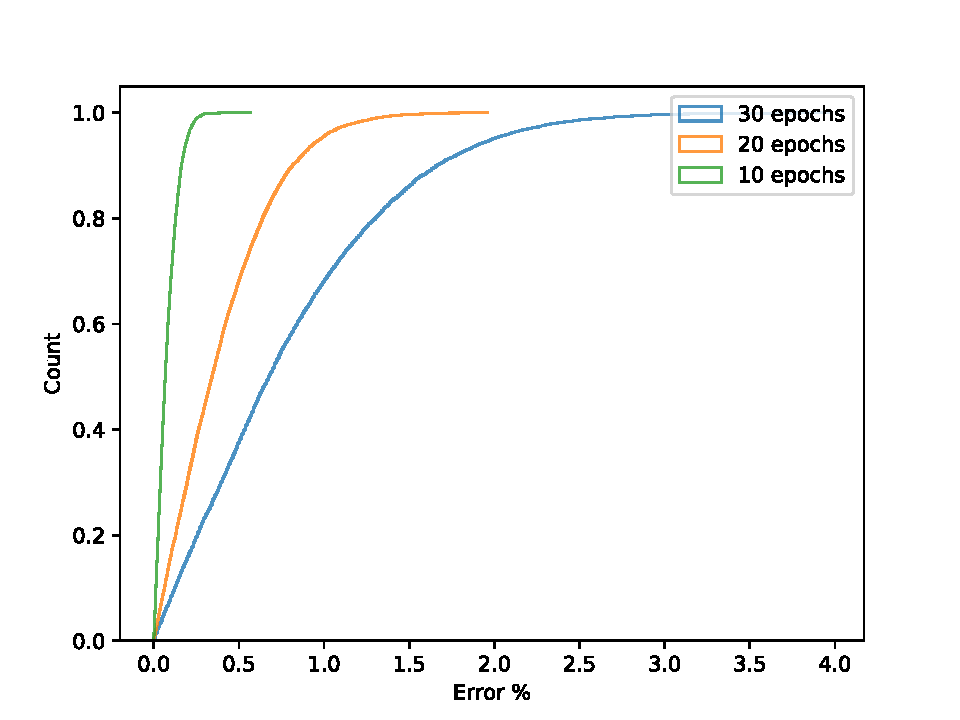
\includegraphics[width=0.9\linewidth]{results/microprofiling_dummy.pdf}
%  \end{subfigure}
%  \caption{\bf\small Errors in accuracy prediction when using Microprofiling. Accuracy errors are higher when predicting for larger number of epochs, but still within xx\% of the true accuracy.}
%  \label{fig:multicam-cities}
%\end{figure}

